\label{sec:docker}
Docker \citep{docker} is a container management tool that packages applications as lightweight containers.
It is already used within the PiCloud on the command line to manage its containers, however monitoring these is a long process based on terminal commands on individual hosts.
Considering the PiCloud has 56 hosts with the possibility of expansion, it would be unreasonable to expect these commands to continue to be done via individual terminal commands, hence the need for \emph{rmt}.
 
 \subsection{DockerUI}
 Docker has an open-source project that provides a web interface which runs client-side so there is the possibility of a user-friendly way to monitor running (or not) containers.
 As can be seen in figure \ref{fig:dockerUiContainers}, the interface shows running containers, the applications those containers are running, and the status of the container.
 This is useful information, however it monitors a single host rather than multiple.

 \begin{figure}[t]
 	\centering
	\setlength\fboxsep{0pt}
	\setlength\fboxrule{0.5pt}
	\fbox{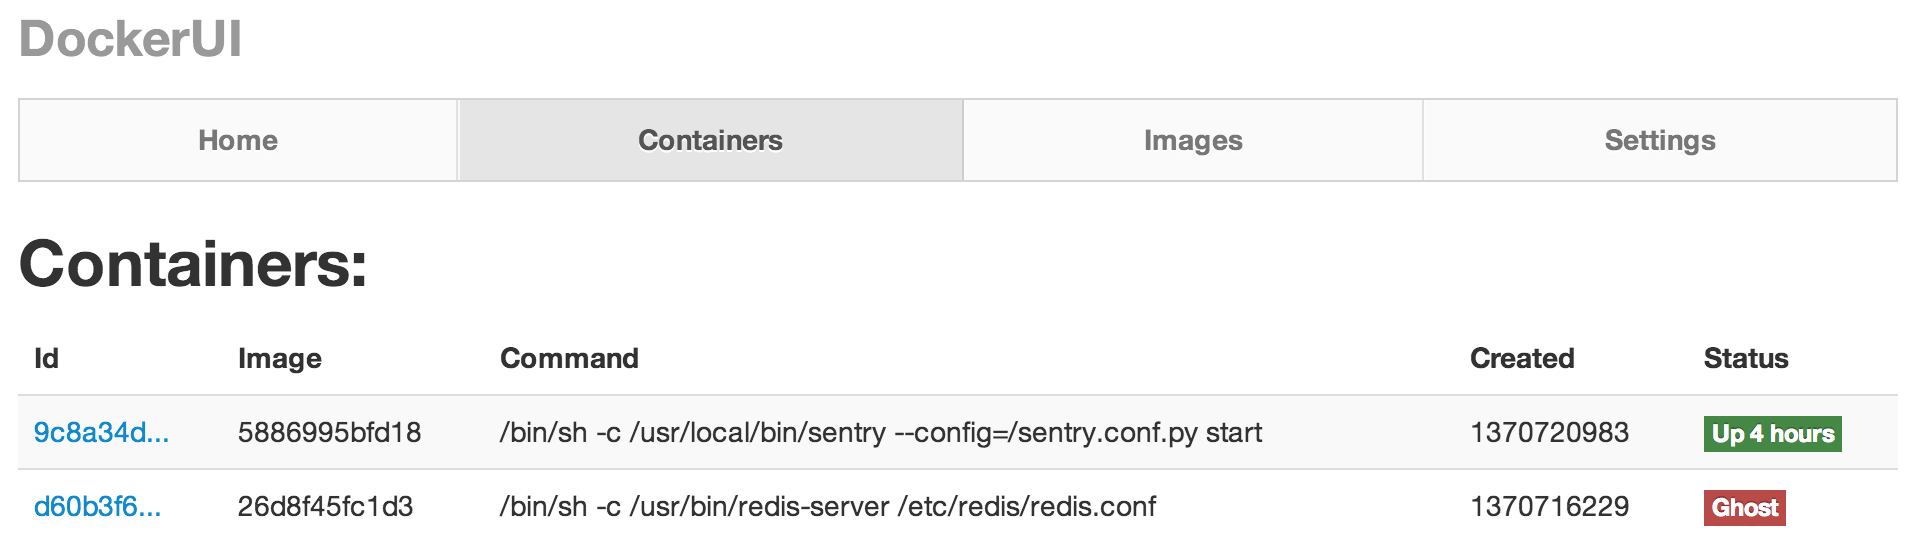
\includegraphics[width=0.8\textwidth]{dockerUiContainers}}
 	\caption{Containers overview in DockerUI}
 	\label{fig:dockerUiContainers}
 \end{figure}

 DockerUI's stated goals are more about wrapping docker functionality into a web app on a single client than acting as a cluster monitor, meaning it is unsuitable for use within \emph{rmt}.
